\documentclass[journal]{IEEEtran}
\usepackage{graphicx}
\usepackage{cite}
\usepackage{multirow}
\usepackage[flushleft]{threeparttable}
\usepackage{booktabs}
\usepackage{siunitx}
\usepackage[T1]{fontenc}
\usepackage[pdftex,breaklinks,pdfauthor={MSD Team P17101},pdfcreator={Philip Linden},pdftitle={P17101 Arcjet Thruster}]{hyperref}
\usepackage{nomencl}
\usepackage{chngcntr}
\usepackage{color}
\makenomenclature{}
% cite.sty was written by Donald Arseneau
% V1.6 and later of IEEEtran pre-defines the format of the cite.sty package
% \cite{} output to follow that of IEEE. Loading the cite package will
% result in citation numbers being automatically sorted and properly
% "compressed/ranged". e.g., [1], [9], [2], [7], [5], [6] without using
% cite.sty will become [1], [2], [5]--[7], [9] using cite.sty. cite.sty's
% \cite will automatically add leading space, if needed. Use cite.sty's
% noadjust option (cite.sty V3.8 and later) if you want to turn this off.
% cite.sty is already installed on most LaTeX systems. Be sure and use
% version 4.0 (2003-05-27) and later if using hyperref.sty. cite.sty does
% not currently provide for hyperlinked citations.
% The latest version can be obtained at:
% http://www.ctan.org/tex-archive/macros/latex/contrib/cite/
% The documentation is contained in the cite.sty file itself.

% http://edge.rit.edu/edge/P17101/public/Home
\title{Multidisciplinary Senior Design P17101: \\ Design of a 1kW Arcjet Thruster}
\author{
  Philip~Linden$^{*}$\thanks{$^{*}$MEng Student, Department of Mechanical Engineering},
  James~Gandek$^{\dagger}$\thanks{$^{\dagger}$BS Student, Department of Mechanical Engineering},
  Dylan~Bruce$^{\dagger}$,
  Matt~Giuffre$^{\dagger}$,
  Anthony~Higgins$^{\ddagger}$\thanks{$^{\ddagger}$BS Student, Department of Electrical Engineering}
}
  % page header for pages other than cover page
  \markboth{P17101 Arcjet Thruster}%
  {Linden \MakeLowercase{\textit{et al.}}: Multidisciplinary Senior Design, RIT}

\begin{document}
\maketitle
% correct bad hyphenation here
\hyphenation{explor-ation explor-atory}

\begin{abstract}
An electrothermal propulsion system was developed for RIT Space Exploration (SPEX) to develop opportunities for design, testing, and characterization of advanced space systems at the Rochester Institute of Technology such as high-efficiency in-space propulsion for station-keeping maneuvers.
% The arcjet thruster demonstrates the degree of practicality in implementing electrothermal propulsion systems.
The thruster assembly generates an electrical arc across the thruster nozzle's throat, ionizing argon propellant in order to achieve a greater specific impulse compared to cold gas propulsion.
\end{abstract}

\label{sec:nomenclature}
% List all symbols and subscripts used for any math equations.
% This will add the units
%----------------------------------------------
\newcommand{\nomunit}[1]{%
\renewcommand{\nomentryend}{\hspace*{\fill}#1}}
%----------------------------------------------
% gas dynamics
% \nomenclature{$A$}{Cross-sectional area of nozzle
%   \nomunit{\,\si{\meter\squared}}}
% \nomenclature{$p$}{Gas pressure
%   \nomunit{\,\si{\kilo\pascal}}}
% \nomenclature{$v$}{Gas flow velocity
%   \nomunit{\,\si{\meter\per\second}}}
\nomenclature{$\dot{m}$}{Mass flow rate
  \nomunit{\,\si{\kilo\gram\per\second}}}
% \nomenclature{$\alpha$}{Diverging nozzle half-angle
%   \nomunit{\,\si{\deg}}}
% rocket equations
% \nomenclature{$F$}{Thrust
%   \nomunit{\,\si{\newton}}}
% \nomenclature{$I_{sp}$}{Specific impulse
%   \nomunit{\,\si{\second}}}
\nomenclature{$g_0$}{Standard acceleration due to gravity
  \nomunit{\,\SI{9.81}{\meter\per\second\squared}}}
\nomenclature{$\sigma_m$}{Mean standard error}
\nomenclature{$\sigma$}{Standard deviation of a sample}
\printnomenclature{}

\section{Introduction}
\label{sec:intro}
\IEEEPARstart{R}{IT} Space Exploration (SPEX) provided a use-case scenario to serve as the basis for this exploration into satellite propulsion.
The mission objective is to design a communications satellite that is capable of maintaining a polar geostationary orbit for 10 years.

In practice, satellites in Earth orbit for long-duration missions (5--25 years) encounter perturbations to their trajectories over time from residual atmospheric and orbital particles, or from variations in Earth's gravity field.
These spacecraft perform short station-keeping maneuvers periodically to compensate for drift and orbital decay.

An electrothermal rocket engine is method of propulsion by which a pressurized inert gas stored at ambient temperature (cold gas) is released and heated electrically before being expelled out of a nozzle.
Two proven methods of electrothermal propulsion are \emph{resistojets}, which use conventional heat exchangers to heat the propellant, and \emph{arcjets}, which pass the propellant through an electrical arc to heat the gas.

Electrothermal propulsion is advantageous over conventional chemical or cold-gas rockets for use by long-life satellites since the engines may be small in size, have no moving parts, and are more efficient at the expense of thrust.
While resistojets and arcjets require more elecrical power than chemical rockets, for example, the electrical energy may be recovered over time by photovoltaic panels whereas propellant fuel is a finite resource for these spacecraft.

A tabletop prototype thruster was designed and tested to explore the feasibility of this type of system with less strict requirements compared to the limitations of building a flight-worthy system.
A tabletop version does not require integration with a spacecraft, and mass and spatial limitations are relaxed.

\section{Design Theory}
\label{sec:method}
% Describe why an arcjet was selected over a resistojet.
In low power (1 kW) applications, an arcjet offers up to 200\% gains in efficiency over a resistojet thruster~\cite{sutton2010rocket}.
\autoref{fig:power-vs-isp} identifies the typical use cases and performance characteristics of arcjets compared to various other types of electrothermal thrusters.
Arcjets achieve a greater specific impulse compared to resistojets but produce less thrust.
Thus a maneuver would take a longer amount of time using an arcjet but would consume less propellant overall for the same maneuver as compared to a resistojet.
\begin{figure}[htp]
  \centering
  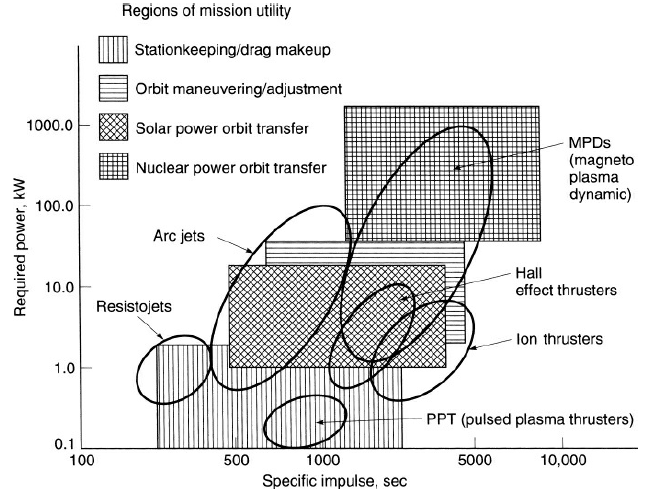
\includegraphics[width=\linewidth]{figs/power-vs-isp_sutton}
  \caption[Types of electrothermal propulsion]{There are various types of electrothermal propulsion with respect to typical performance and mission utility.
  In the \SI{1}{\kilo\watt} range, arcjets typically have a higher specific impulse than resistojets. (Sutton~2010)
\label{fig:power-vs-isp}}
\end{figure}

% Justify propellant selection (and explain paschen curve?)
The ideal propellant for arcjet engines is one which can be stored for long periods of time, has a low atomic mass, and favorable thermodynamic conditions during heating and expansion.
NASA identifies Hydrogen (H$_{2}$), Ammonia (NH$_{3}$), and Hydrazine (N$_{2}$H$_{3}$) as ideal propellants for arcjets~\cite{nasa1992considerations}.
Unfortunately, these gases are toxic or difficult to handle on a university campus.
Nitrogen (N$_{2}$) is an easy-to-handle alternative that has relatively favorable ionization and thermodynamic characteristics, and has been used in similar low-power arcjet demonstrations~\cite{olin2012report,olin2012sim}.
Argon (Ar) is a very cheap, easy-to-handle, and highly available alternative to these propellants, and has similar characteristics regarding breakdown voltage and ionization energy.
Argon was selected for testing since it was available for student use on RIT's campus.
% High level gas dynamics analysis
\begin{figure}[htp]
  \centering
  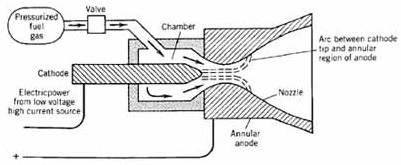
\includegraphics[width=\linewidth]{figs/cross-section_nasa}
  \caption[Arcjet cross-section]{A cross sectional view of a typical arcjet shows the expected flowpath of propellant and the expected region of the electric current arc. The propellant is ionized and heated by the arc then expanded through the nozzle. (NASA~GRC~1992)
\label{fig:x-section-nasa}
}
\end{figure}

Gas enters the chamber and is ionized and heated by a high-current arc that extends from the cathode to the throat of the anodic nozzle to form a plasma.
The plasma reaches sonic speed in the throat and is supersonically accelerated as it expands through the nozzle.
% Ideal flow performance is illustrated in \autoref{fig:flow-graphs}, assuming
% uniform flow across nozzle cross sections, isentropic flow conditions (except across shocks), zero vorticity, and unmoving flow at inlet.

% \begin{figure}[htp]
%   \centering
%   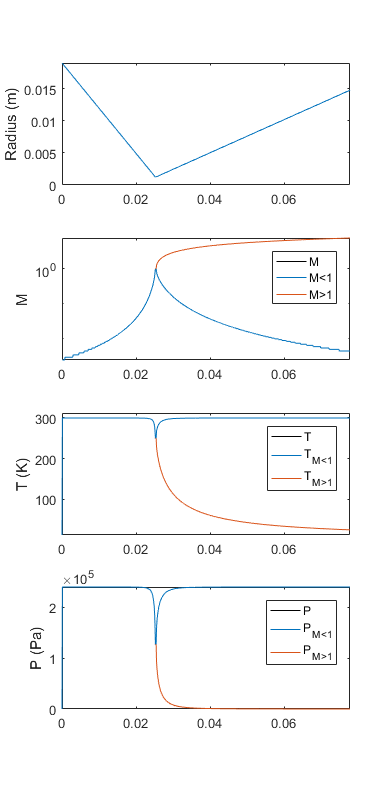
\includegraphics[width=\linewidth]{figs/flow.png}
%   \caption[P17101 Arcjet Annotated Cutaway]{{\color{red}Update with predicted flow through nozzle, including shocks.}
% \label{fig:flow-graphs}
% }
% \end{figure}

Thrust is a function of the momentum of the flow exiting the nozzle, which is primarily driven by the pressure ratio between the total pressure of the propellant at the inlet and environmental pressure at the nozzle's exit.
Greater environmental pressures decrease the performance of the nozzle, especially considering it is designed for space operation.
\begin{equation}
\label{eq:thrust}
  F=\dot{m}v_e + (p_e-p_b)A_e
\end{equation}
 Where $F$ is thrust, $\dot{m}$ is mass flow rate of propellant, $v$ is flow velocity, $A$ is nozzle cross sectional area of the nozzle, and subscript $e$ denotes parameters at the nozzle exit while $p_b$ denotes atmospheric backpressure.
 In space, $p_b$ is negligible and the thruster is design around such condition.

 A thruster's efficiency is described in terms of specific impulse, $I_{sp}$, which may be used to compare performance with other space propulsion methods.
 \begin{equation}
 \label{eq:isp}
   I_{sp}=\frac{F}{\dot{m} g_0}
 \end{equation}

The goal of ionizing the gas is to add energy with electricity such that the momentum of the exhaust is greater for the same amount of mass, thus improving the efficiency of the thruster.
% some calculations?
% In the ideal condition using gaseous N$_2$ as propellant, a conical nozzle with $\alpha=15$ is capable of {\color{red}\SI{0}{\newton} of thrust} without a sustained arc.
% At sea-level, {\color{red}\SI{0}{\newton} of thrust} is expected.

% \begin{table}[hbp]
%   \caption{Theoretical thrust and $I_{sp}$ values with respect to space and sea-level operation, total pressure $p_0= $\SI{239.2}{\kilo\pascal}.
% \label{tab:theoretical-performance}
% }
% {\color{red}
%   \begin{tabular}{lrrrrr}
%     \toprule
%     & & \multicolumn{2}{c}{Without arc} & \multicolumn{2}{c}{With arc} \\
%     & $p_b$ (\si{\kilo\pascal}) & Thrust (\si{\newton}) & $I_{sp}$ (\si{\second}) & Thrust (\si{\newton}) & $I_{sp}$ (\si{\second}) \\
%     \midrule
%     Vacuum    & $0$     & $0$ & $0$ & $0$ & $0$ \\
%     Sea-level & $101.3$ & $0$ & $0$ & $0$ & $0$ \\
%     \bottomrule
%   \end{tabular}
%   }
% \end{table}

The thruster was simulated for the cold gas case without an electric arc using the SolidWorks Flow Simulation computational fluid dynamics package, shown in~\autoref{fig:flowsim}.
As shown in the simulation, the cold gas does not reach sonic speed at sea-level pressures.
Without an arc, the flow does go supersonic in a vacuum, but not enough to provide sufficient thrust to a spacecraft.
Exit velocity is shown to increase with an increase in inlet pressure as well.

The behavior of the gas in response to an electric arc was not possible to model in SolidWorks, and the heat transferred to the gas by the arc is difficult to model analytically~\cite{mitarcjets}.
The team decided to observe effects of introducing an arc to the flow empirically.

\begin{figure}
  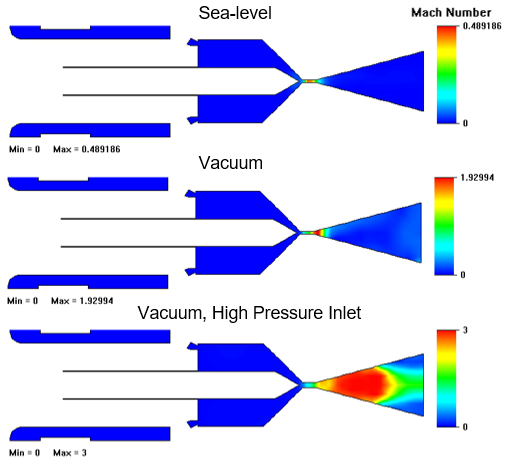
\includegraphics[width=\linewidth]{figs/flowsim}
  \caption{Nitrogen gas was simulated without the electric arc through the nozzle with SolidWorks Flow Simulation.
  \emph{Top: }\SI{20}{psi} inlet pressure, \SI{1}{atm} (sea-level) environmental pressure.
  \emph{Center: }\SI{20}{psi} inlet pressure, \SI{0.1}{atm} (near-vacuum) environmental pressure.
  \emph{Top: }\SI{200}{psi} inlet pressure, \SI{0.1}{atm} (near-vacuum) environmental pressure.}
\label{fig:flowsim}
\end{figure}

\section{System Overview}
% outline the main system architecture.
\subsection{Thruster}
% Describe the main components of the thruster and how they interact. Be sure to include material selection justifications. Show some basic analysis and predictions for performance with justification.
Propellant flows into a stainless steel body and is spun into a vortex about the tip of the cathode, where it passes through an electric arc before being accelerated through a conical nozzle.
The flow swirler doubles as a high-temperature ceramic insulator.
The insulator and cathode are mounted concentrically into a low-temperature PTFE thermal and electrical insulator, which is fixed to the thruster test stand via toe clamps.
The nozzle is electrically insulated from the steel body by a non-conductive alumina spacer.

% how much energy transferred from arc to plasma?
\begin{figure}[htp]
  \centering
  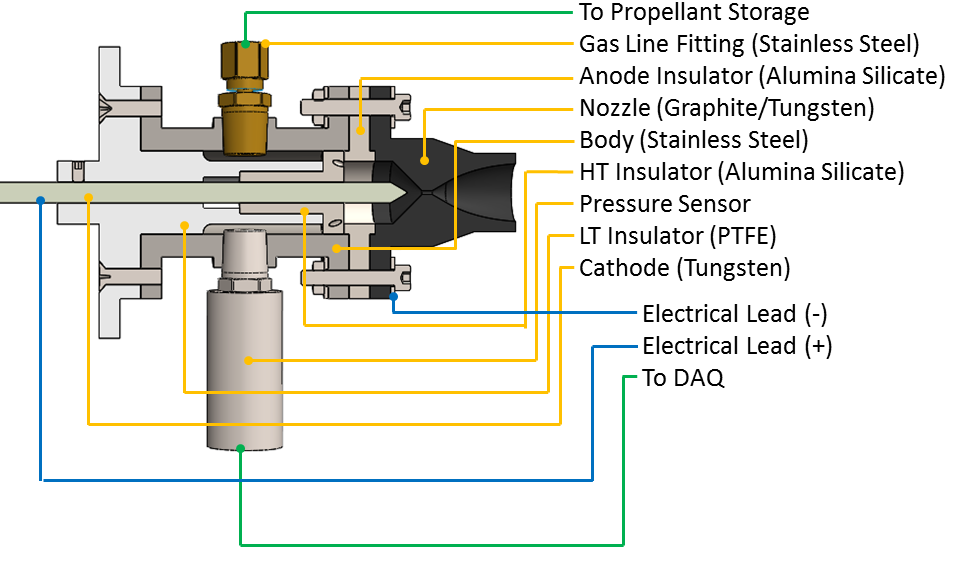
\includegraphics[width=\linewidth]{figs/cutaway_annotated.png}
  \caption[P17101 Arcjet Annotated Cutaway]{Components that are charged or exposed to extreme heat are electrically and thermally insulated.
\label{fig:annotated-cutaway}
}
\end{figure}

\subsection{Power Conditioning Unit}
% Describe the inputs and desired outputs of the unit. Explain the theoretical justification behind the HV/HC approach. Describe the approach in theoretical terms and list practical limitations.
The electrical arc used to add energy to the gas is generated and sustained by the Power Conditioning Unit (PCU).
The PCU consists of separate high-voltage (HV) and high-current (HC) sides.
The HV side of the circuit initiates the arc, then the PCU switches to the HC ``side'' of the circuit to sustain a high-current arc.
This architecture is similar to a plasma torch and has been demonstrated in similar tabletop systems~\cite{park2015thesis}.

% explain HV side here
\SI{120}{\volt} AC power is supplied to the PCU from a standard wall outlet.
The HV side of the circuit raises the voltage by several orders of magnitude.
The small capacitor and dimmer switch send a signal to the ignition coil to generate a HV low current arc similar to a spark plug.
This arc is created between the small auxilary copper electrode in the alumina silicate insulator and the main tungsten electrode and ``primes'' the gas to reduce the breakdown voltage.
The HV arc allows the larger capacitor and power resistors to discharge an HC arc, that ionizes the gas and forms a plasma between the main tungsten to the graphite nozzle.
When performing properly all subsequent gas must flow through this plasma, imparting heat, and therefore energy that leads to better performance than a cold gas configuration alone.
This current passes through a coil that activates a reed switch, turning off the HV side of the PCU.\@

\begin{figure}[htp]
  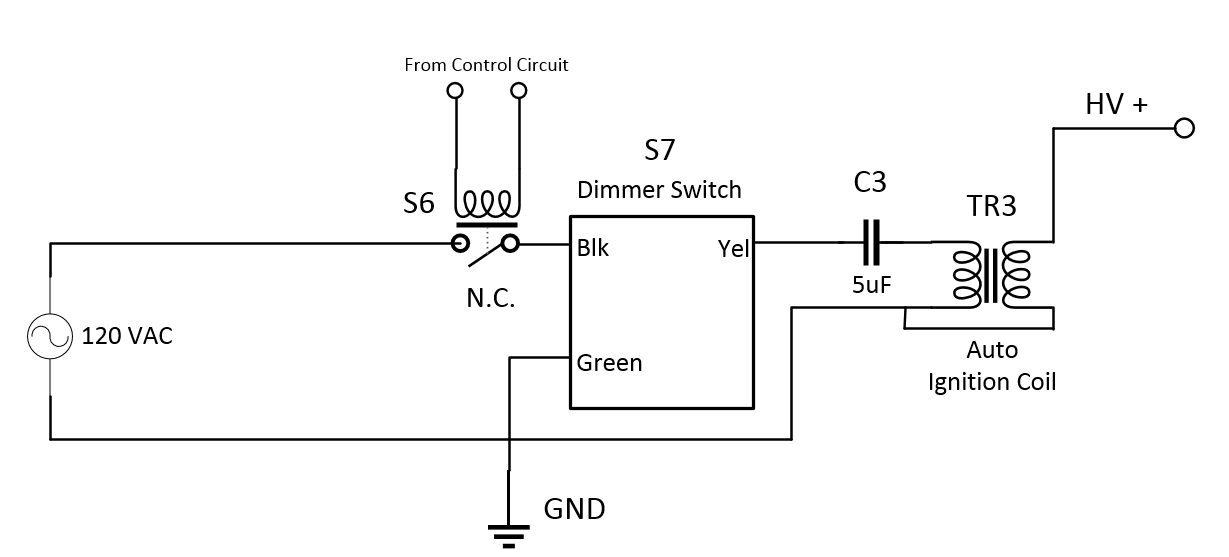
\includegraphics[width=\linewidth]{figs/hv-schematic.png}
  \caption{Wall AC power is converted to DC high voltage in order to initiate an arc.
\label{fig:hv-circuit}
}
\end{figure}

% explain HC side here
The control circuit for the high current works by utilizing a lower voltage DC source.
To achieve this, the \SI{120}{\volt} AC signal is passed through a step down transformer and is rectified to DC.\@
A normally open reed switch is used to detect current passing through the coil in the HC circuit.
When closed, the DC voltage is applied to the relay in the HV circuit.
The relay is normally closed, so applying a voltage to it disables the HV side.

\begin{figure}[htp]
  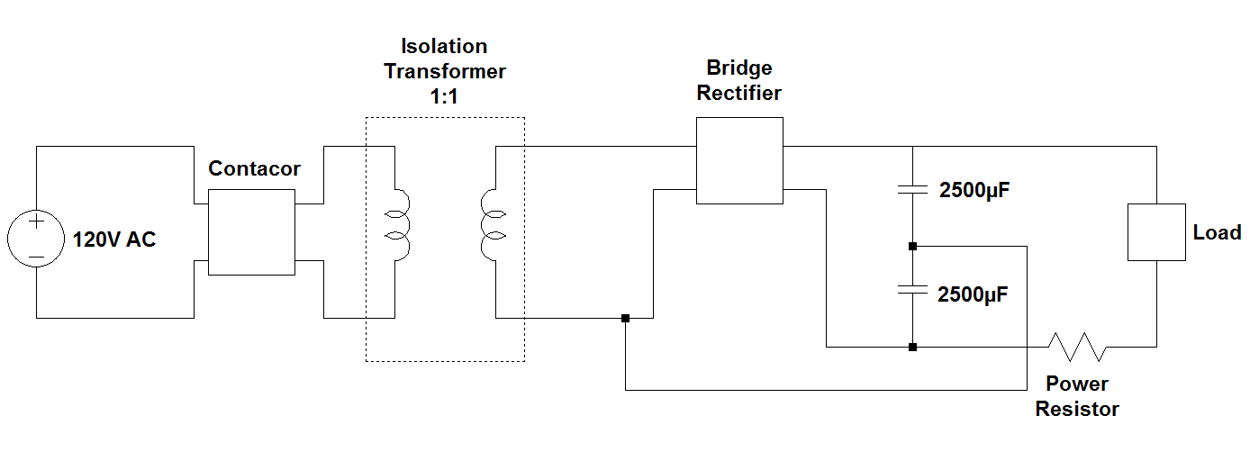
\includegraphics[width=\linewidth]{figs/hc-schematic.png}
  \caption{A schematic of the components used in the HC circuit.
  The 120V AC line from the wall gets rectified into a DC voltage with a power resistor controlling the current draw.
\label{fig:hc-circuit}
}
\end{figure}

The HC circuit works by rectifying the \SI{120}{\volt} AC sine wave, resulting \SI{170}{\volt} DC.\@
The arc closes the circuit, allowing electrons to flow.
The high current is drawn from heating coils acting as power resistors.
The two heating coils can be configured to have a resistance of \SI{7.5}{\ohm}, \SI{15}{\ohm}, or \SI{30}{\ohm}.
All tests were performed with the \SI{15}{\ohm} configuration.
The HC circuit has a coil that activates a reed switch when on.
The reed switch activates a relay which turns off the HV circuit.

The PCU is housed in a modified computer server chassis shown in~\autoref{fig:pcu-annotated}.
This provides a grounded area with many tie-down points for electrical components to be placed.
Clearance holes for component stakes are drilled through the panels and components are secured with screws, cable ties, and 3M double sided tape
Two desktop computer case fans are mounted in the back of the PCU housing to provide some airflow to cool the power resistors during operation.

During nominal operation, the PCU draws $1700$--$1800$\si{\watt} from the wall outlet.

\subsection{Test Stand}
% Explain the physical apparatus that measures the system's outputs. Describe the interactions between the thruster and the test stand. Justify instrumentation selection.
The test stand, shown in~\autoref{fig:teststand-annotated}, is cantilevered in design, leveraging both the mass of the thruster and its operating thrust.
Because expected thrust output is less than \SI{50}{\milli\newton} and load cells in this range are either very costly or lack the necessary accuracy, the thruster mass is used as an offset that suits a more common range load cell.
The resolution of a 0--6\si{\kilo\gram} Omega LCAE-6kg load cell was chosen as a reasonable middle ground between load resolution and cost.

The construction of the stand is largely 6061-T6 aluminum with the test platform assembled to an oil-impregnated bronze rod that allows for displacement vertically downwards on the load cell.
Two 6''$\times$8'' plates are welded at a right angle with a pair of gussets to form the main structure of the stand, and two bearing blocks are fastened several inches further up to capture the bronze bearing rod and test platform itself.
The thruster is mounted to the test platform using a set of three toe-clamps to make the set up and breakdown of the system simple and efficient.
The stand's construction allows for some variability in expected test results through a set of slots used to position the load cell. Since it offers a small form facto, the complete mechanical system can be accommodated in a range of different testing environments such as the engine test cell that is used to complete these initial studies.

\begin{figure}[htp]
  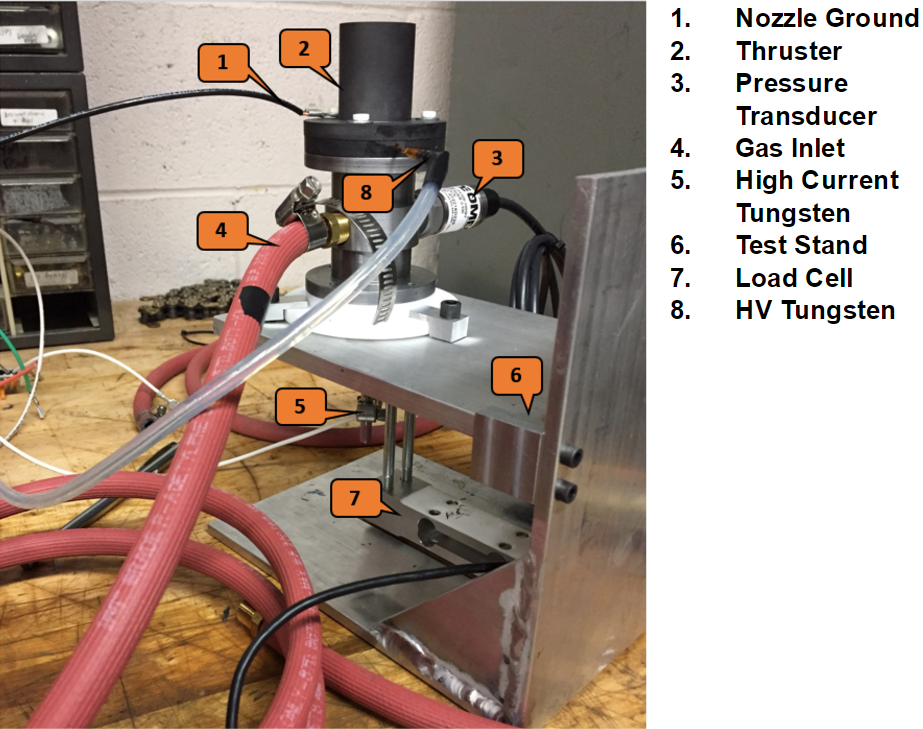
\includegraphics[width=\linewidth]{figs/teststand-annotated.PNG}
  \caption{An annotated view of the thruster assembly and test stand in the test configuration.
  \emph{Not shown:} A compressed gas dewar with an inline flow meter and regulator valve are connected to the gas inlet tube (4) prior to the solenoid valve.
\label{fig:teststand-annotated}
}
\end{figure}

\begin{figure}[htp]
  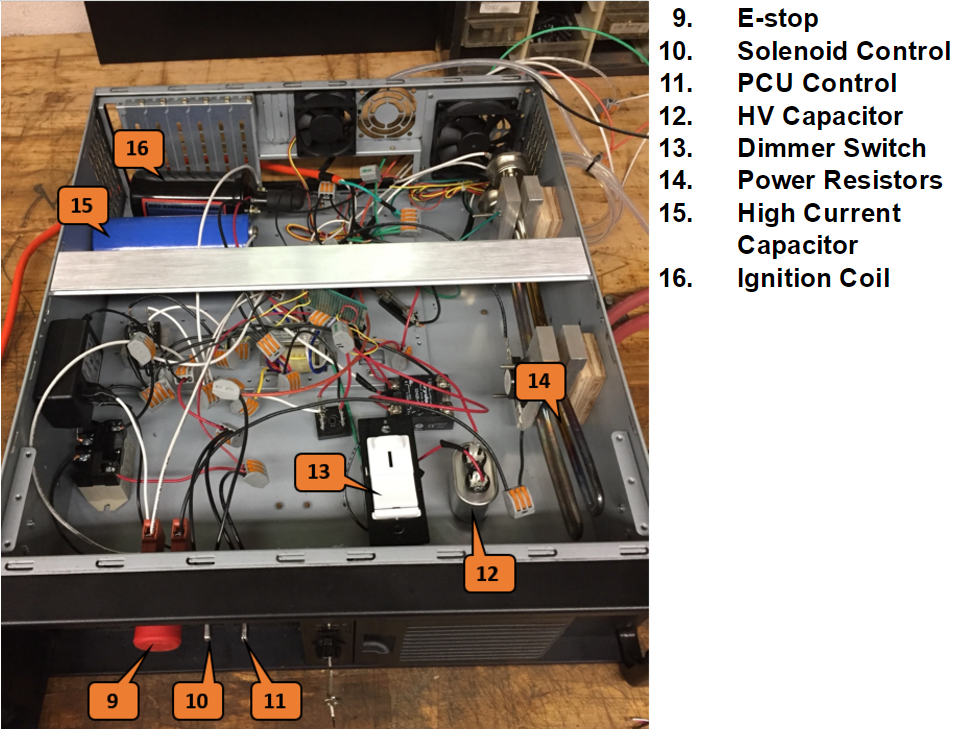
\includegraphics[width=\linewidth]{figs/pcu-annotated.PNG}
  \caption{An annotated view of the open PCU.\@
  Small components such as relays are not labeled here for clarity.
  The the top cover of the PCU housing (not shown) may be installed to enclose the system completely.
\label{fig:pcu-annotated}
}
\end{figure}

Propellant is supplied by a compressed gas dewar at \SI{2200}{psi}.
The gaseous argon is nominally regulated to \SI{20}{psi} before reaching a normally-closed solenoid valve.
Argon is flowed through the system for several seconds before PCU ignition to ensure only propellant is present in the thruster, and after PCU shutdown to help cool hot thruster components.

The propellant solenoid and PCU are activated and deactivated toggle switches next to an emergency shut-off button, shown in~\autoref{fig:pcu-annotated}.

\subsection{Data Acquisition \& Control}

Data acquisition (DAQ) is collected by a National Instruments MyDAQ device utilizing a LabVIEW Virtual Interface (VI).
Two DAQ devices were recognized as being readily available, the NI USB-6008 and the NI MyDAQ.\@
The USB-6008 device offers more overall channels (4 analog input) but with a much lower throughput (\SI{10}{kS/s}) and resolution (12-bit).
The MyDAQ device only offers 2 analog input channels but offers \SI{200}{kS/s} at 16-bit resolution. It was determined that the primary performance metric would be the thrust force generated during a burn with pressure inside the main body being a secondary performance metric.
Acquiring data for these metrics would only require two analog input channels and as such, the MyDAQ device was chosen for its superior precision.
Both devices were also capable of generating an output which would be sufficient to actuate the transistors, which in turn activate the PCU and propellant solenoid, so this parameter was not taken into consideration during device selection.
Initially the DAQ was configured to send control commands to activate and deactivate the PCU and solenoid, but this was later removed due to errors encountered during testing. Toggle switches were then mounted to the front of the server chassis to manually control the solenoid and PCU.

The test engineer starts and stops recording a test data set with the VI
 % (see~\autoref{fig:VI-frontpanel})
from a computer connected to the test stand.
Once the proper channels are selected for data acquisition (analog inputs), the DAQ parameters may be chosen (i.e.\ sample rate \& number of samples per channel).
The test engineer may also choose whether to save test data.
After a data set is collected, it is displayed on an amplitude versus time plot.

\subsection{Safety Measures}
% Describe risk management in more detail. Consider ommitting this section~\cite{linden}.
Several safety measures were included in order to mitigate the risk in operating the system. A thermal cut-off switch opens in the main power line at a temperature of \SI{250}{F} and re-closes at \SI{210}{F}. In the event of a computer malfunction, an emergency shutoff button is wired into the circuit between the outlet and the PCU and the solenoid is normally closed and non-latching.
This emergency shut-off and the toggle switches used to engage the PCU and solenoid are mounted behind a locking door such that the emergency shut-off button is pressed when the door is closed.
The safety door is closed whenever the system is not in use, and locked when the system is stored.

When a test is conducted, the test stand is placed in a ventilated dynamometer test cell, and the control computer is located outside the testing room.
The VI monitors sensor data in real-time and shuts down operation when sensor parameters reach unsafe limits, and may be stopped via the stop button on the front panel or by the satisfaction of a number of safety interlocks present within the block diagram.
Examples of these interlocks are errors in the DAQ sequence, positive gauge pressure present in the thruster's main body before starting the VI, or a ten second timeout.

% Because of some charring observed in the plywood base during circuit operation, an informal test was performed on the power resistors under operational conditions to gain an estimate on the temperature changes over time.
% The graphs below show the average temperature increase is 7.4F per second. The charring temperature of wood is 250-300F, and a 10s burn would require a temperature buffer of 80-90F.
% In order to protect the wood enclosure a temperature cutoff was added to the power line that opens at 250F.

\section{Test Procedure}
% Describe the basic test plan in broad terms and how we approached testing. Describe the setup within the engine test cell and how the user interacts with the system.
The test stand, PCU, and propellant supply canister are placed in an engine test cell located in the RIT Department of Mechanical Engineering Machine Shop.
This space is typically used for engine testing and is outfitted with reinforced doors, walls, and windows, a ventilation system, and an adjacent room fitted with computers.
The arcjet thruster assembly is in view of the computer room windows.
Wires for data acquisition and control are fed from the National Instruments myDAQ device, and are connected to a computer running the DAQ VI.\@

The thrust load cell is calibrated in the test configuration by placing precision masses at the thrust location on the nozzle and recording at least 3 data sets for each calibration load.
The calibration loads are used to correlate output voltage from the load cell into force data.

% \begin{figure}
%   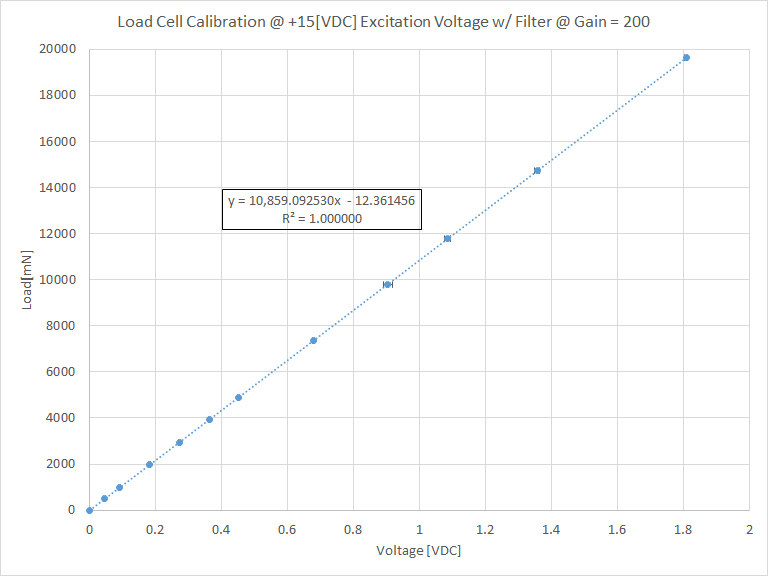
\includegraphics[width=\linewidth]{figs/loadcell-cal.png}
%   \caption{Using multiple data sets for a range of known precision mass loads, output voltages from the load cell are averaged and a calibration curve is drawn.
% \label{fig:loadcell-cal}
% \end{figure}

For each test, the test cell doors are closed to minimize outside noise and as a protection measure.
The propellant solenoid valve opens one to two seconds before the PCU engages to purge air from the system to ensure only propellant is present in the thruster.
The PCU ignites the arc and sustains it for at least five seconds.
The PCU disengages and cold gas continues to flow for an additional two to five seconds in order to cool the thruster.
The solenoid valve closes and the system is safed via the emergency shut-off.
Thrust and pressure data are saved to a tab-delimited text file.

Load cell data was collected for no operation, cold gas only, and gas flow with the PCU engaged.
The data set for no operation is used to tare the thrust scale and allow the weight of the system to be filtered out of other test data sets.
By collecting thrust data for cold gas only and with the PCU engaged, the effects of adding heat to the gas with an electric arc may be assessed.
For each data set, volumetric flow rate was measured by a flow meter in-line and downstream from the propellant supply.

\section{Results}
\subsection{Qualitative Performance}
% Show results and how they compare to our pred|ictions. Describe any failures and the problem solving process that occurred.
The thruster was unable to completely ionize the gas when operating at the \SI{1}{\kilo\watt} power limit originally imposed on the project. In order to achieve consistent ionization, one of the two power resistors originally included in the circuit was removed in order to double the power and current flowing through the system. This updated schematic with only one power resistor is shown in~\autoref{fig:pcu-schematic}. After doubling the power from \SI{925}{\watt} to \SI{1850}{\watt}, the PCU consistently generates and sustains an electric arc that spans from the tungsten electrode to the graphite nozzle.
Using argon or nitrogen propellant, the gas is ionized and hot plasma is ejected from the nozzle, as shown in~\autoref{fig:burn-snapshots}.
When supplied flow rate exceeded 25 cubic feet per hour (CFH), the exhaust remained partially ionized.
When flow rate was limited to 22\si{CFH}, the exhaust appears to be fully ionized.
This could be due to the gas partially choking in the throat of the nozzle, and not fully reaching sonic speed until specific conditions are reached.

\begin{figure}
  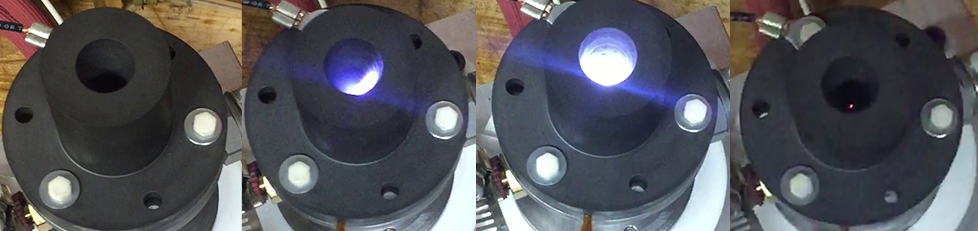
\includegraphics[width=\linewidth]{figs/burnsnapshots.png}
  \caption{Videos were recorded during test fires.
  \emph{Far left:} The system before a test.
  \emph{Center left:} The arc is generated and the propellant is partially ionized.
  \emph{Center right:} A fully realized plume of plasma is sustained in the nozzle.
  \emph{Far right:} After 5--10 seconds of thrust, the PCU is deactivated and the tungsten electrode glows red hot while the graphite nozzle is warm to the touch.
\label{fig:burn-snapshots}}
\end{figure}

\subsection{Quantitative Performance}
Empirically, the true thrust load is lost in measurement error, primarily due to a 10\% error in the load cell (Omega LCAE-6KG).
Per Omega's instruction, calibrations were performed to remove this 10\% error, however after several different iterations of calibration, the results varied significantly and occasionally were not even linear, as shown in~\autoref{fig:curve}.
Without a clear calibration to follow, the best method toward obtaining results was to create a linear trend of the useable calibration data and to bound that trend with a 95\% confidence interval, both in slope and intercept.
The trend and interval were both calculated using MATLAB software's curve fitting toolbox, shown in~\autoref{tab:cal}.

\begin{table}
  \centering
  \caption{95\% Confidence Bounds on Omega LCAE-6KG Calibration
\label{tab:cal}}
  \begin{tabular}{lcc}
    \toprule
    & Intercept (\si{\volt}) & Slope (\si{\volt\per\milli\newton}) \\ \midrule
    Estimate & 1.911 & 0.001082 \\
    Upper Bound & 1.914 & 0.001152 \\
    Lower Bound & 1.908 & 0.001011 \\
    % \midrule
    % Mean     & $-22.8$\tnote{b} & $ $ & $15.0$ & $ $  \\
    \bottomrule
  \end{tabular}
\end{table}

Voltage output from the load cell is noisy, but oscillates symmetrically about values to a precision of $\pm10\%$ in accordance with the manufacturer specification.
On the millinewton scale, load cell measurement data is very noisy, and signal noise worsens while the PCU is engaged.
% estimated thrust below \SI{50}{\milli\newton}.
% So 50mN was always going to be beyond the reach of this load cell, then?
%
% Matt Giuffre [< 1 minute ago]
% Beyond the reach of any load cell costing < $3000
Additional measurement error is suspected to be caused by electromagnetic interference from the high-voltage components operating in close proximity to telemetry cables.

A Kaiser window FIR filter was applied to the data to smooth out noise spikes.
Some large spikes were not removed by the filtering, so windows were then also applied to ensure clean data.
An example of the unfiltered and filtered data, as well as the windows applied to remove the remaining anomalies is shown in~\autoref{fig:raw-data}.
The results of filtering the calibration and cold-fire data is shown in~\autoref{fig:other-raw-data}.
While the filter did smooth out the results for these conditions, it left a large amount of low-frequency sinusoidal noise.
This filtering did not adjust the averages of these data sets significantly, and so these data sets were left unfiltered for analysis in order to be computationally efficient.

% Low-frequency vibrations from the environment itself may also play a role since the test stand is located within the RIT Kate Gleason College of Engineering machine shop, where numerous lathes, mills, and other heavy machinery operate.
% FS = 6kg = 6000g = 58860mN
% 58860mN * ±10% = ±5886mN
% Since we gave the sensor a gain of 200:
% FS = 38000mN
% 38000mN * ±10% = ±3800mN
% Q.E.D.
% but even if you achieve ±1% FS, that gives you ±380mN
% {\color{red}Observation data was filtered using?.
% The designed filter removes much of the high frequency ($>100$\si{Hz}) noise present in the signal, but low frequency noise remains present.}
% % Matt Giuffre [9:04 PM]
% % It's a Kaiser window FIR filter. It essentially a very aggressive gaussian window. It attenuates at -60dB/decade at the stopband as opposed to the -20dB/decade which is standard. This is because I assumed the data to be relatively steady
% A filtered tare load for the system with no gas flowing through the nozzle is shown in \autoref{fig:tare-data}.

\begin{figure}
  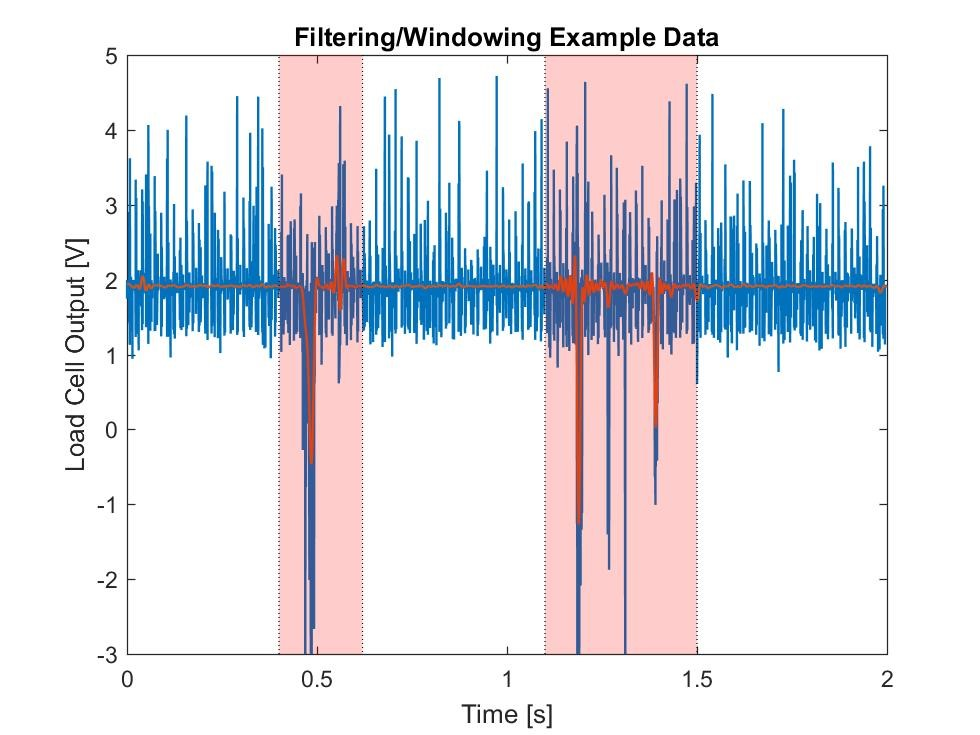
\includegraphics[width=\linewidth]{figs/raw-data.jpg}
  \caption{Example two-second data set showing results of both filtering and windowing. Removed sections are highlighted in red.}
\label{fig:raw-data}
\end{figure}

\begin{figure}
  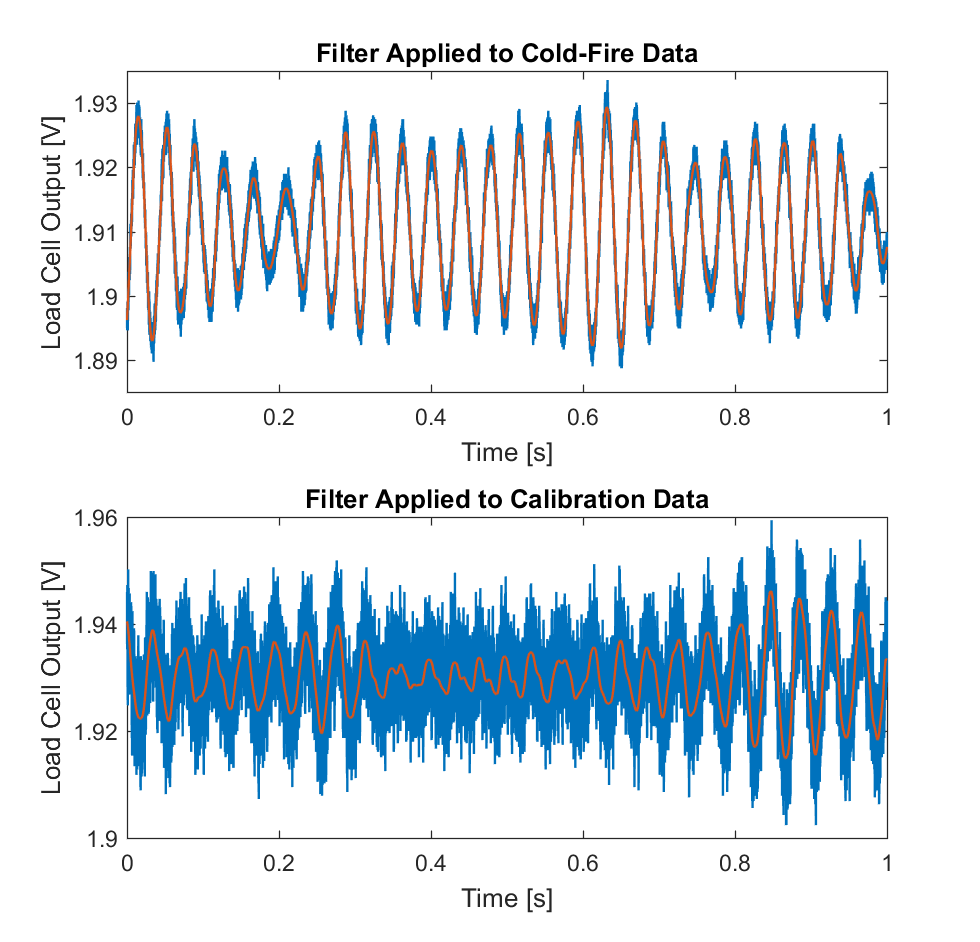
\includegraphics[width=\linewidth]{figs/other-raw-data.png}
  \caption{One second sets of calibration and cold-fire data showing results of filtering on sinusoidal noise.}
\label{fig:other-raw-data}
\end{figure}

In each of four rounds of testing, three two-second tests at 100,000 data samples per second were taken of the thruster firing, and four two-second tests at 100,000 data samples per second were taken of cold gas firing.
Each data set was averaged and these averages are shown in~\autoref{tab:test-means}.

\begin{figure}
  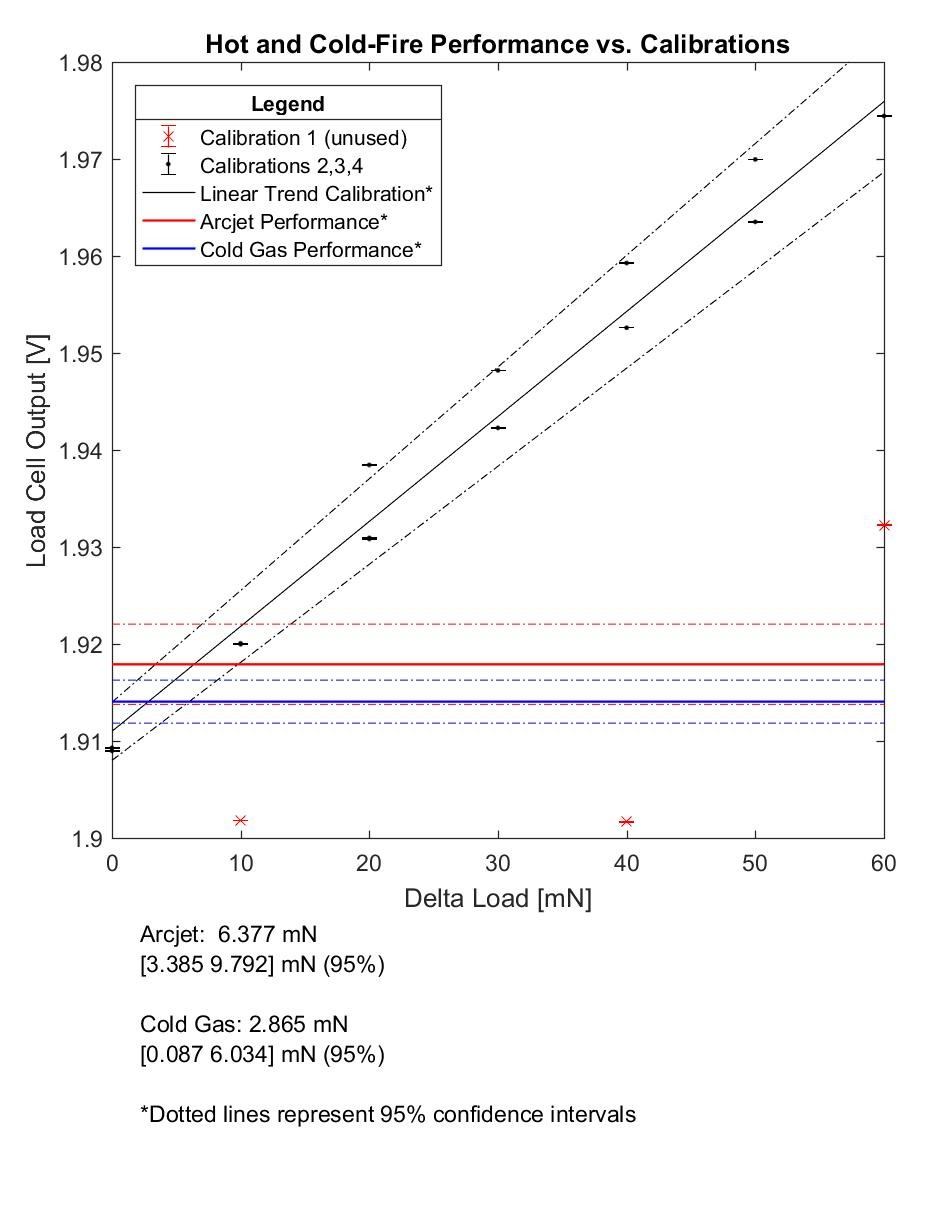
\includegraphics[width=\linewidth]{figs/thrust-data.jpg}
  \caption{95\% Interval for output voltage from the load cell plotted against 95\% calibration interval.}
\label{fig:curve}
\end{figure}

\begin{table}
  \centering
  \caption{Voltage means for hot-fire and cold-fire tests
\label{tab:test-means}}
  \begin{tabular}{rcc}
    \toprule
    Test & Hot-Fire (with arc) & Cold-Fire \\ \midrule
    1 & 1.9287 & 1.9195 \\
    2 & 1.9192 & 1.9172 \\
    3 & 1.9097 & 1.9103 \\
    4 & 1.9131 & 1.9092 \\
    \bottomrule
  \end{tabular}
\end{table}

To obtain the thrust average and errors of each test condition, the mean output voltages of all 12 hot-fire and all 16 cold-fire tests were averaged separately, and a 95\% error bound for each test condition was created using 1.96 times the standard error of each group.
These errors for sample size N were calculated as
\begin{equation}
\label{eq:stderr}
  \sigma_m = \frac{\sigma}{\sqrt(N)}
\end{equation}
These means and standard errors are plotted as horizontal lines on~\autoref{fig:curve}, which can then be traced back to where they meet with the linear calibration.
For the lower bound of thrust, the lower bound of each test condition voltage is matched with the upper bound of the linear calibration, and for the upper bound of thrust the upper bound voltage of each test condition is matched with the lower bound of the linear calibration.
This provides an range of thrust values taking into account 95\% confidence on both the test measurements as well as the calibration itself.

Metrics on the true performance of the thruster is inconclusive.
Claiming thrust and specific impulse results from these data would be highly uncertain and potentially misleading.
However, the data shows that thrust for tests with and without the arc engaged are statistically different.
While the true performance can not be quantitatively determined, it is clear that the qualitative goal of achieving a change in performance over cold gas propulsion by ionizing propellant with an electric arc has been met.

% \begin{figure}
%   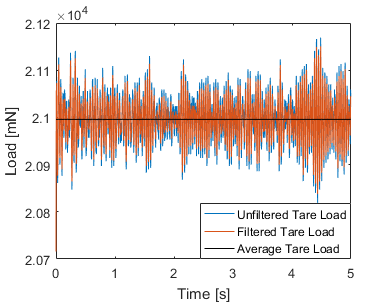
\includegraphics[width=\linewidth]{figs/tareload.png}
%   \caption{.}
% \label{fig:data-noise-psd}
% \end{figure}

% \begin{figure}
%   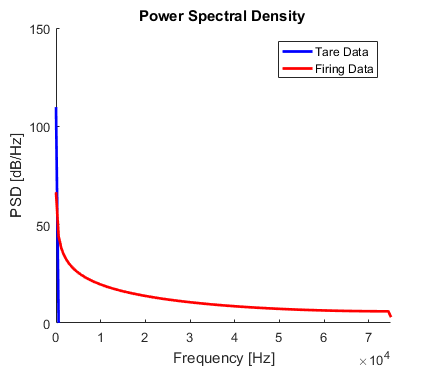
\includegraphics[width=\linewidth]{figs/data-noise-psd.png}
%   \caption{For data collected in the tare case, noise in the load cell data does not extend beyond 0--\SI{0.1}{Hz}.
%   During a test fire with the PCU engaged, the power spectral density of the load cell data is significant from 0--\SI{75}{\kilo{}Hz}.
%   Since the system should physically reach a steady state condition relatively quickly, the oscillations must be attributed to noise in the load cell output signal.}
% \label{fig:data-noise-psd}
% \end{figure}

\section{Conclusions}
The system was visually observed to be ionizing the gas in operation. The characteristic glows of nitrogen and argon were both seen during testing with each respective gas, and so qualitatively the system achieves its goal of ionizing propellants.

The exhaust gasses were observed to partially ionize when supplied propellant flow rate exceeded \SI{22}{CFH}.
Coupled with the heat addition by electric arc in the throat of the nozzle, this indicates that the flow may be partially choked under some uncontrolled test conditions.
The current test stand and instrumentation package do not provide sufficient data to determine if the flow becomes fully choked at the nozzle's throat.
If the exhaust is partially choked, then some of the gas flow reaches sonic speeds while other regions do not, and this scenario may only be modeled computationally.

While it is impossible to draw exact thrust values from the data collected, the difference in measured thrust between the hot-fire and cold-fire test conditions is significant.
In three out of four rounds of testing, the hot-fire condition out-performed the cold-fire condition.
Using MATLAB software, a null hypothesis of both overall data sets coming from populations with equal means is rejected at the 1\% significance level by both a standard T-test as well as a Kruskal-Wallis test of variance.
Since the data sets were taken sequentially, this suggests there is a consistent difference between the average thrust measured under each condition.
An important point to note is that these hypothesis are rejected by combining all raw cold-fire data into one set, and all filtered hot-fire data into one set.
If the same tests are run on arrays containing the means of each individual data set, the null hypothesis cannot be rejected as there is approximately a 22\% chance of each sample coming from populations with the equal means.
As arcjet technology has been well researched and this has previously been shown to be the case, this result is consistent with other published research and the teams expectations.

Should the calibration trend and thrust averages hold, the thrust benefit of hot-fire over cold is
\begin{equation}
  \Bigg(\frac{6.377 \text{[mN]}}{2.865 \text{[mN]}} - 1\Bigg)\times100\% = 122\%
  \end{equation}
This is similar in magnitude to the 200\% gain claimed by previous arcjet thruster systems~\cite{sutton2010rocket}.
However, due to the noise and error present in the system and measurements, this number cannot be claimed as a true result.
More testing and more precise measurements are needed to discern the actual change in thrust and specific impulse over cold-gas propulsion.

\section{Recommendations}
% Evaluate the success of the project and make recommendations for improving it.
\subsection{Data Acquisition}
Ultimately, in order to obtain accurate and repeatable results regarding the thrust output of the arcjet system, a more precise force transducer must be used.
Since NASA's estimate for thrust output of the arcjet is on the order of \SI{50}{\milli\newton}, the ideal sensor should have a systematic uncertainty on the order of $\pm$ \SI{5}{\milli\newton}.
The NI myDAQ device provides an adequate sampling rate and resolution for this task, and as such would not need to be substituted.
The downfall of the data acquisition portion of this application is primarily due to the use of an imprecise instrument.
The sensor used had a force rating of \SI{6}{\kilo\gram} $\pm$ 10\%, whereas the ideal solution would be to use a sensor with a maximum rating of \SI{1}{\kilo\gram} $\pm$ 0.5\% or similar.
Low force sensor such as this, however, cost in excess of \$1000 and as such were deemed too expensive for the budget of this project.

Shielded wire could be used to prevent electrical noise, however the noise in the hot-fire data files was successfully filtered out and the dominant noise in cold-fire test data was sinusoidal vibrations around \SI{30}{Hz} from the machine shop environment.
Reducing or eliminating these vibrations would significantly improve test accuracy.

\subsection{Telemetry and Test Environment}
Robust characterization of the thruster would only be possible with improved sensors, not only for thrust but also for temperatures of the gas and physical system.
It may be possible to show in-space performance by testing the system in a low-pressure environmental chamber.

The oil-impregnated bronze used as a rotational shaft in the test stand design seemed to function adequately, but a ball-bearing design would be more appropriate and might reduce any possible rotational friction.

\subsection{Thruster Design}
The high-voltage electrode was late in the design once it became clear it was needed to prime the gas.
Consequently, the alignment hole drilled through the side of the insulator was a very temporary fix.
If the placement of the HV electrode in the disc insulator is to remain in the future, either the insulator should be thickened, or another local insulation method should be pursued to prevent unwanted arcing that was sometimes observed between the HV electrode and the nozzle or stainless steel body.

The flow rate observed during testing was 20--25\si{CFH}.
This is higher than what is reported in similar systems and could end up limiting the maximum specific impulse of the thruster.
Interestingly, there was little observed difference between a nozzle with a \SI{.050}{in} diameter throat and a nozzle with the \SI{.025}{in} diameter throat.
% A third nozzle could be made with an \SI{.013}{in} throat ($\#$80 drill) to see if the flow can be more effectively limited.

Ideally, nozzle design should be driven by theoretical performance based on analysis or simulation.
The team recommends development of a robust theoretical model of the flow and heat transfer in this electrothermal system to inform future development.
The ideal nozzle profile would choke the flow prior to the diverging section, and diverge along a spline rather than a conical section.


\subsection{Control and Circuitry}
Originally, the PCU and solenoid were designed to be controlled by MOSFET via a \SI{5}{\volt} output signal from the DAQ, thus allowing the operator to be in a different room than the test setup.
The MOSFETs selected consistently shorted over the course of testing for unknown reasons.
Given when this problem was identified, toggle switches were judged to be an acceptable risk to get the system properly functioning in time.
In the future, a more robust control circuit would allow remote activation as originally intended and would lead to much safer operation.

While the hot water heater elements served adequately as power resistors, they heated up extremely quickly (\SI{15}{\celsius\per\sec}) and warped under thermal load.
The heater elements have a finite lifespan in air, and a more permanent cooling or other resistive solution could be designed in the future.


\section*{Acknowledgments}
The team thanks Mr.~Vincent Burolla and Dr.~Dorin Patru for their unwavering support; the Mechanical and Electrical Engineering Departments, the Multidisciplinary Senior Design Department, and the Kate Gleason College of Engineering for their resources and workspaces; RIT Space Exploration and The Boeing Company for sponsoring this project.

\bibliographystyle{IEEEtran}
\bibliography{p17101}


\onecolumn
\appendices{}
\counterwithin{figure}{section}
\section{PCU Schematic}
\begin{figure}[h]
  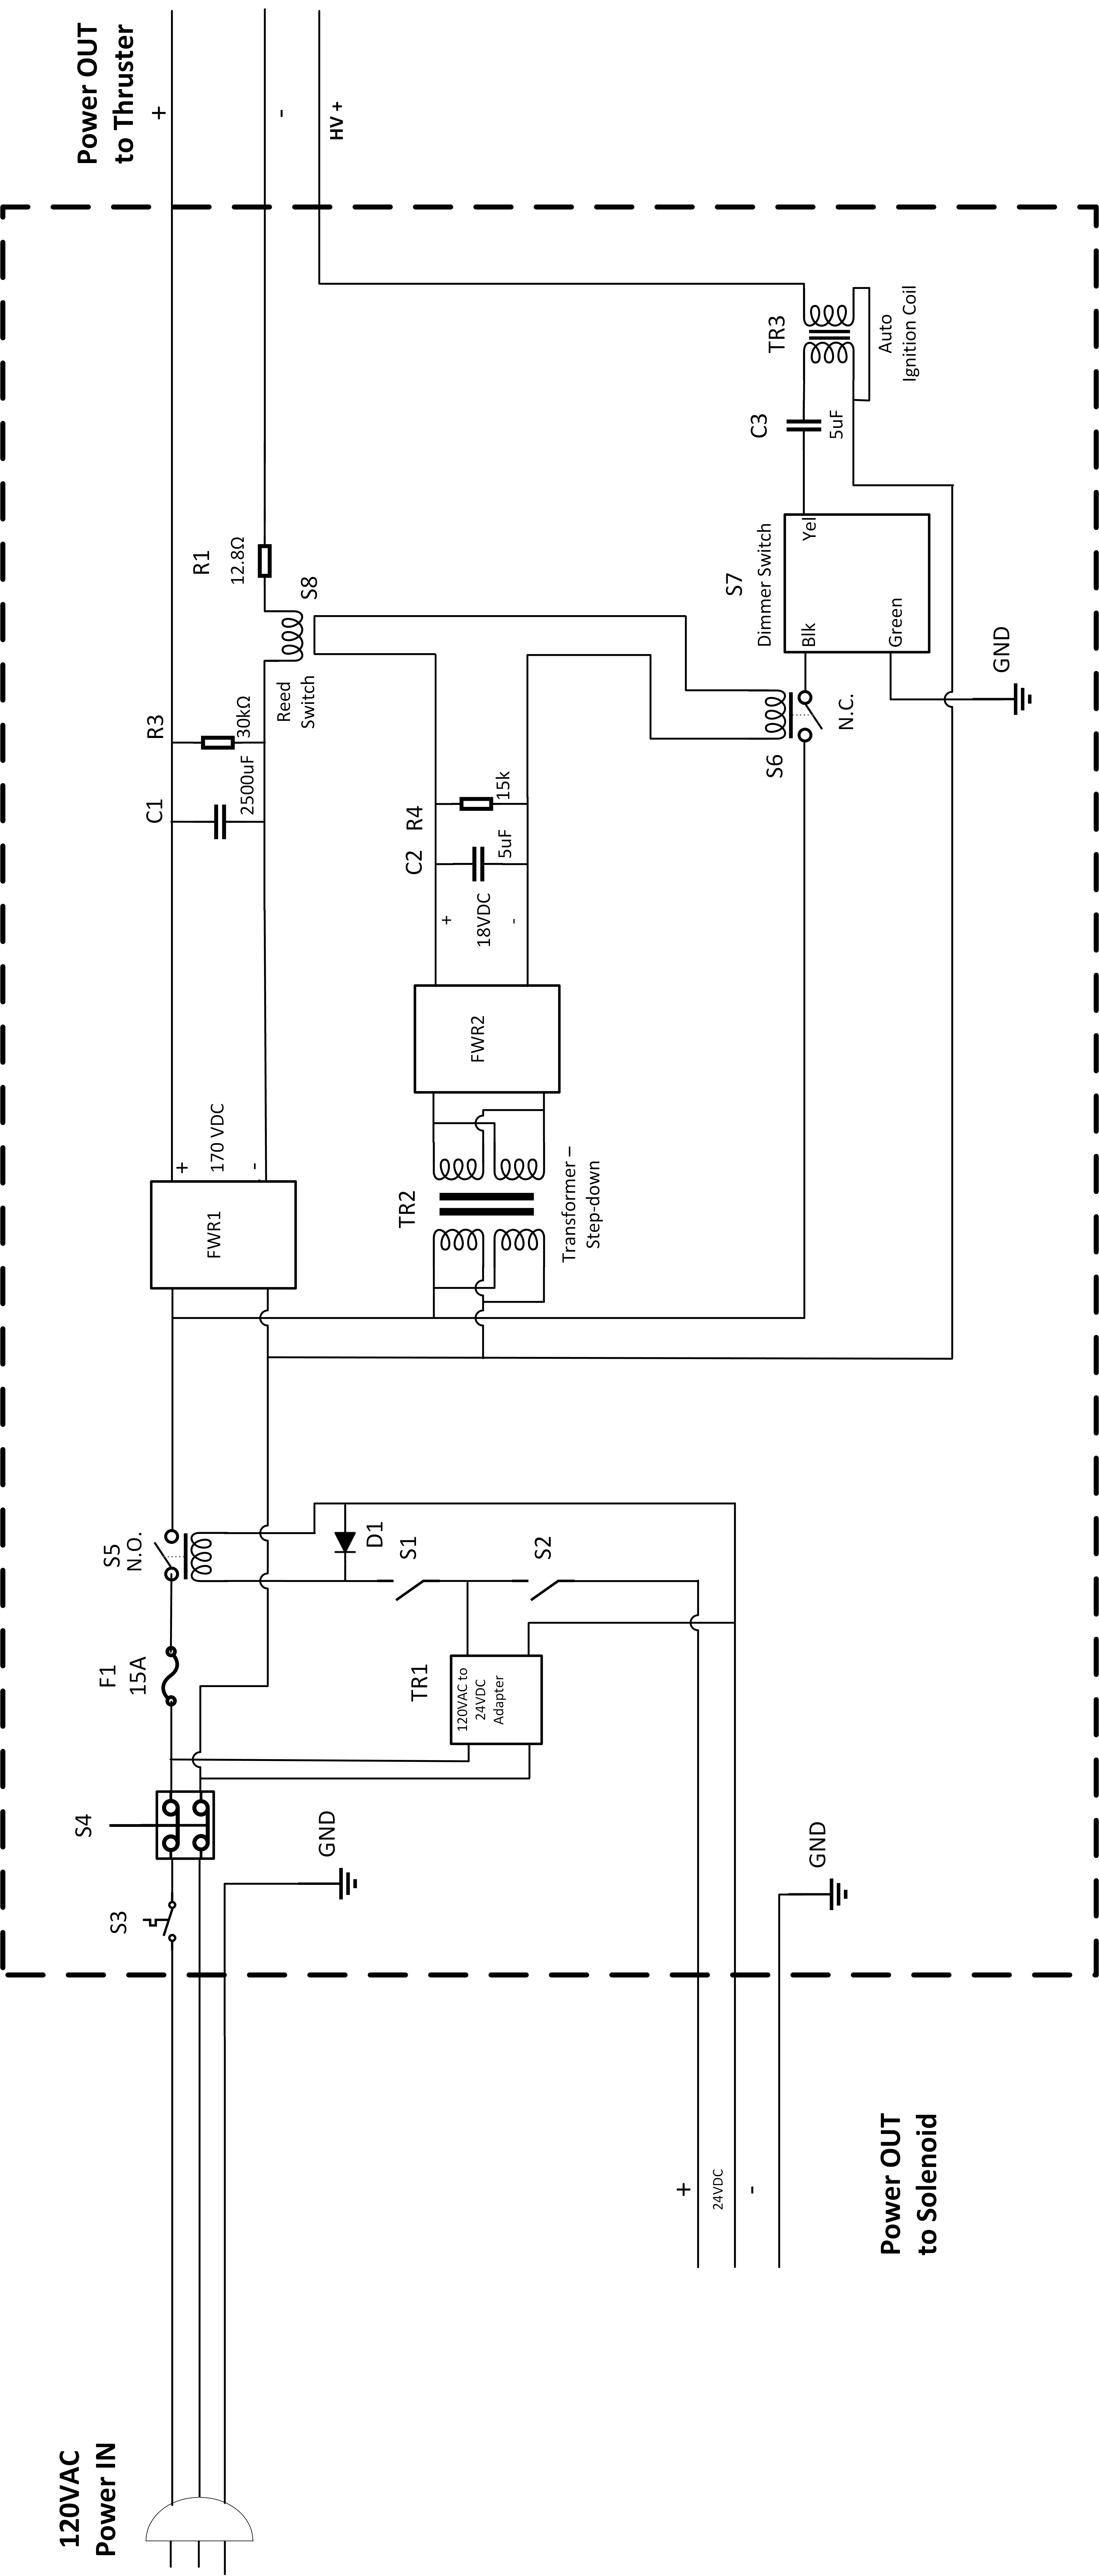
\includegraphics[height=.8\vsize,keepaspectratio]{figs/PCU_Schematic_No_AI_4_27_rotated.png}
  \caption{Electrical diagram of the PCU.}
\label{fig:pcu-schematic}
\end{figure}

%\section{Data Aqcuisition \& Control Virtual Interface}
%% Images will need to be updated once proper data acquisition/recording and safety interlocks are implemented.
%\begin{figure}[htp]
%  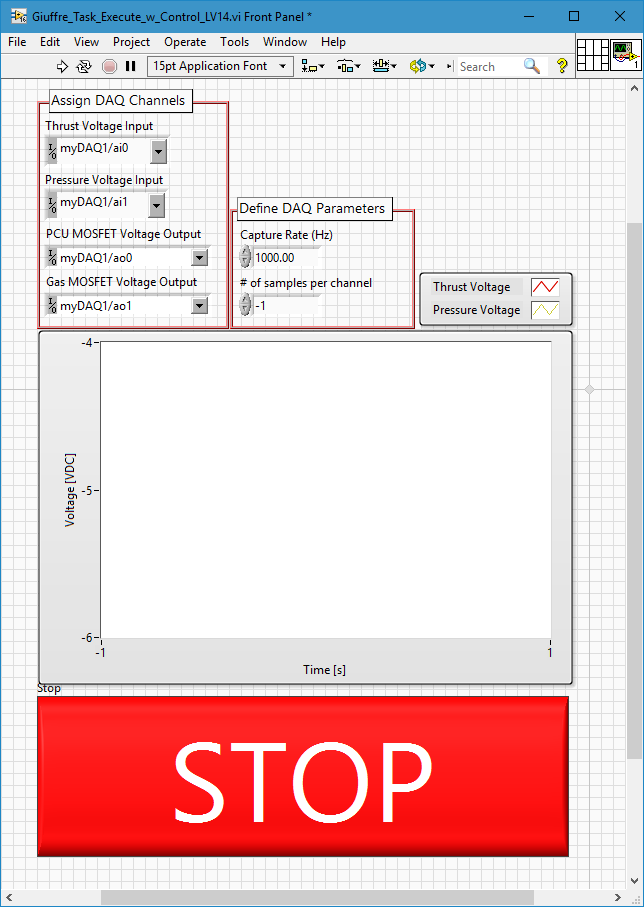
\includegraphics[height=.6\vsize,keepaspectratio]{figs/VI_30Mar17_FP.png}
%  \caption{The user interface for the DAQ/Control VI.\@
%\label{fig:VI-frontpanel}
%}
%\end{figure}

% \begin{figure}[htp]
%   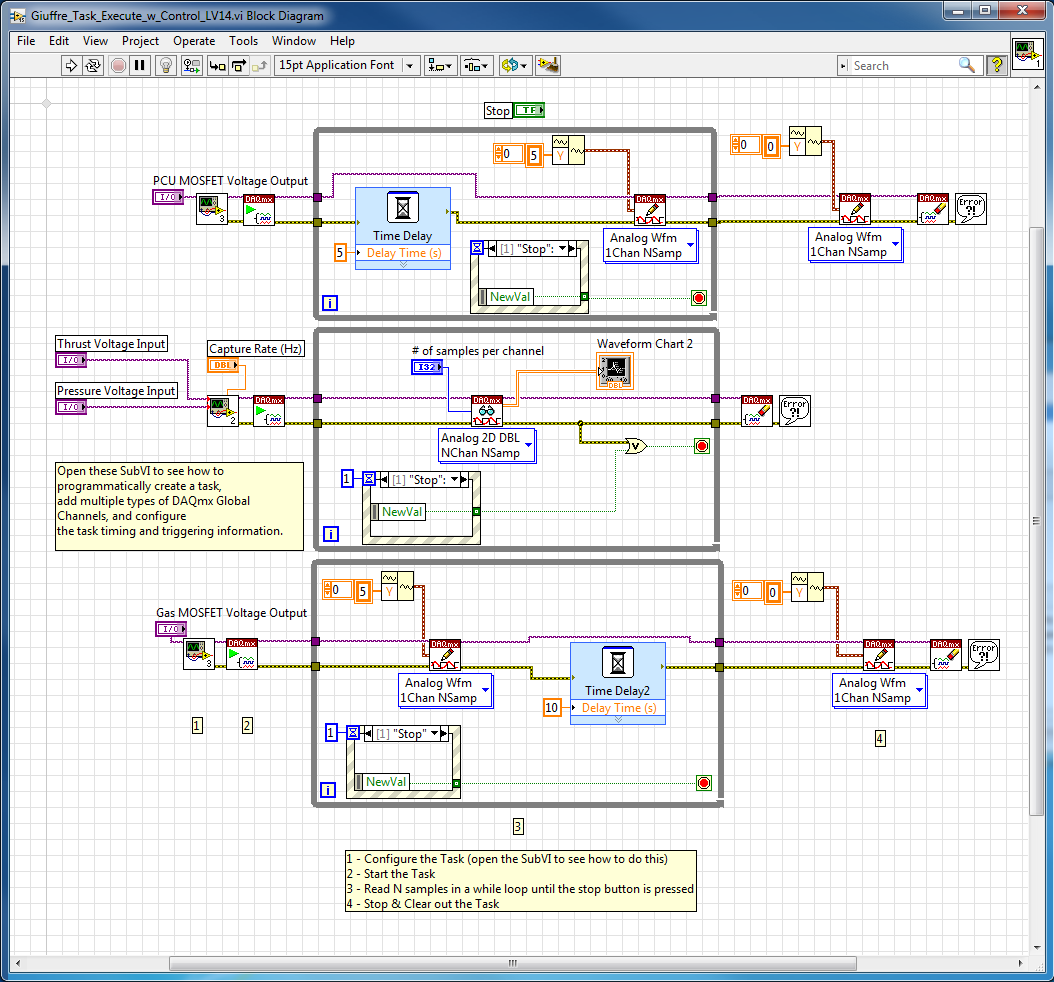
\includegraphics[height=.5\vsize,keepaspectratio]{figs/VI_30Mar17.png}
%   \caption{The block diagram for the DAQ/Control VI.\@
% \label{fig:VI-blockdiagram}
% }
% \end{figure}
%
% \begin{figure}[htp]
%   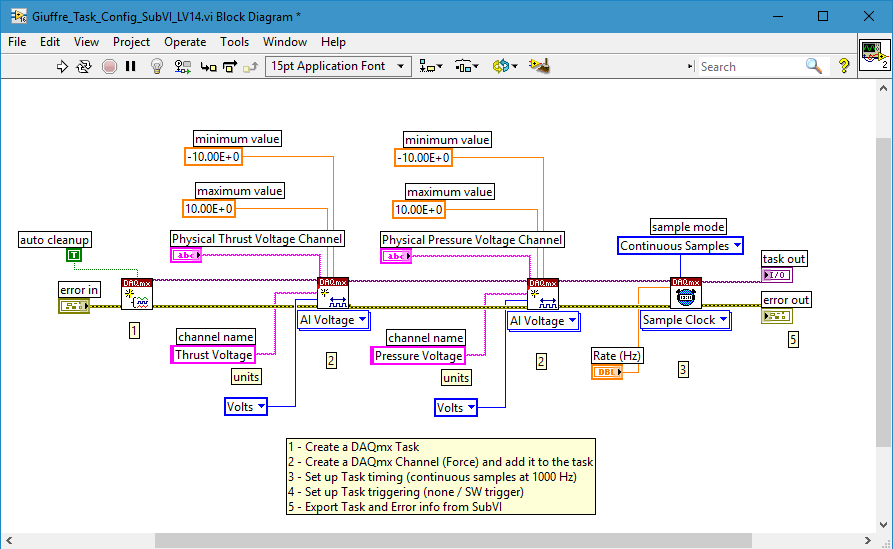
\includegraphics[height=.4\vsize,keepaspectratio]{figs/VI_30Mar17_SubVI.png}
%   \caption{One of three sub-VIs used within the main VI to define channels \& tasks.
% \label{fig:VI-subVI}
% }
% \end{figure}
\end{document}
